\chapter{SNAP}

Esta clase tiene como objetivo familiarizarse con el entorno gráfico del \emph{Sentinel Aplication Toolbox (SNAP)}. El SNAP es el software de procesamiento de imágenes diseñado por la \emph{Agencia Espacial Europera (ESA)}. Este tiene distintas herramientas que simplifican el trabajo con imágenes radar y ópticas, además de la realización de procesamiento de imágenes en general.

\section{Interfaz gráfica del SNAP}

Descomprima los archivos decargados que se denominan \path{material.tar.gz}. Abra el programa SNAP, allí encontrará la interfaz gráfica del usuario (Figura \ref{fig:int})

\begin{figure}[h!]
    \centering
    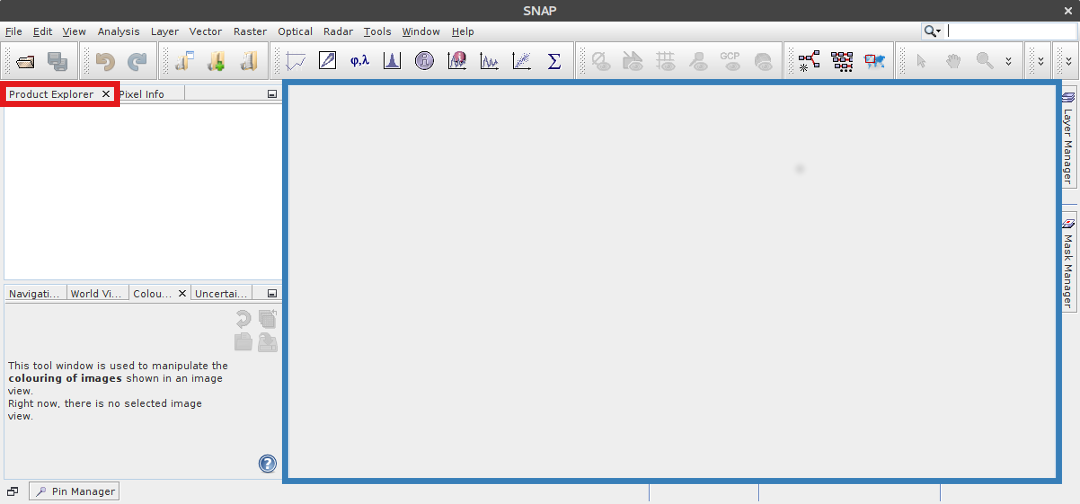
\includegraphics[scale=1.1]{fig:int.png}
    \caption{Interfáz gráfica del usuario. El \emph{Producto Explorer} y el área de visualización del programa.}
    \label{fig:int}
\end{figure}

\section{Apertura de imágenes}

En el menú principal, seleccione \emph{Open product...} y dentro de la carpeta \path{material/raster_data}, seleccione \path{S2A_USER_MTD_SAFL2A_PDMC_20161206.dim}.

Haga doble click sobre el nombre de la imgen y se desplegará un árbol que incluye las siguientes opciones:
\dirtree{%
    .1 [1] S2\_MSIL2A\_20170702.
    .2 Metadata.
    .2 Index Codings.
    .2 Vector Data.
    .2 Bands.
    .2 Masks.
}

En esta cobertura encontramos

\begin{itemize}
    \item \emph{[1] S2\_MSIL2A\_20170702}: El número de elemento entre corchetes, que marca en que orden se abrieron los productos y el nombre de la imagen.
    \item \emph{Metadata}: Los metadatos asociados a la imagen y su historial de procesamiento.
    \item \emph{Index Codings}: Los valores de referencia para interpretar los números digitales de la imagen.
    \item \emph{Vector data}: Las capas vectoriales asociadas a la imagen.
    \item \emph{Bands}: Las bandas de la imagen y las operaciones de álgebra entre bandas.
    \item \emph{Masks}: Las máscaras que sean incluidas en la imagen.
\end{itemize}

\section{Visualización}

Para visualizar una de las bandas de la imagen haciendo doble click sobre ella. La banda se mostrará en escala de grises (Figura \ref{fig:mono})

\begin{figure}[h!]
    \centering
    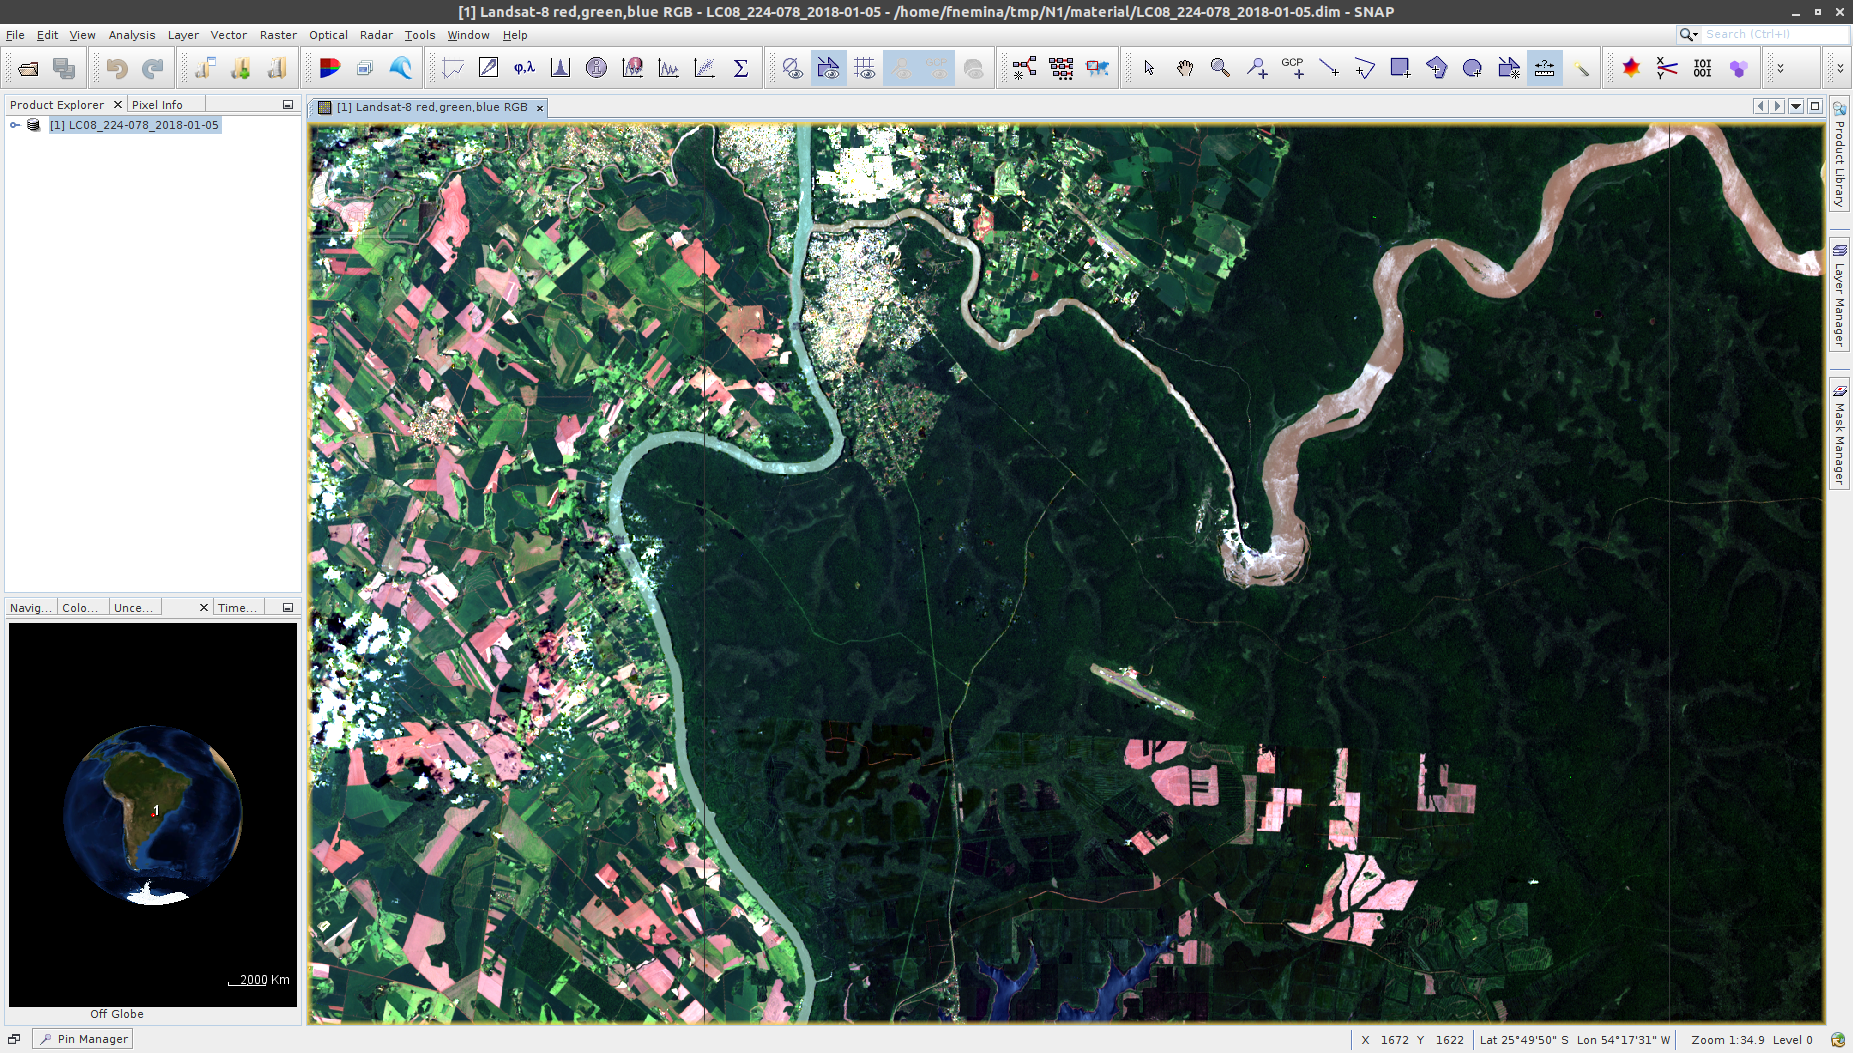
\includegraphics[scale=0.7]{fig:mono.png}
    \caption{Imagen monobanda desplegada en el visualizador.}
    \label{fig:mono}
\end{figure}

Es posible abrir varias bandas en simultaneo, cada una de ella se mostrará en una pestaña nueva arriba del área de visualización.

Explore la imagen utilizando las herramientas de navegación y zoom (Figura \ref{fig:NAV})

\begin{figure}[h!]
    \centering
    
\includegraphics[scale=0.5]{fig:NAV.png}
    \caption{Herramientass de navegación. De izquierda a derecha: \emph{Selection tool}, para seleccionar objetos en la imagen, \emph{Panning tool}, para moverse dentro de la imagen, y \emph{Zooming tool}, para hacer zoom en la imagen.}
    \label{fig:NAV}
\end{figure}

En el \emph{Product Explorer} haga click derecho sobre el nombre y seleccione \emph{Open RGB image windows}. Se desplegará una nueva ventana (Figura \ref{fig:RGB}) que le permitirá elegir la combinación de bandas.

\begin{figure}[h!]
    \centering
    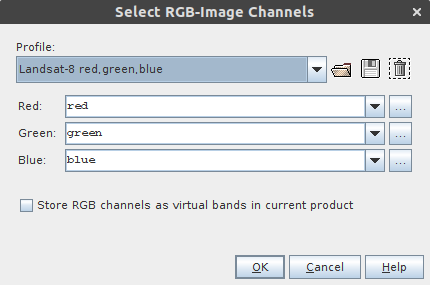
\includegraphics[scale=0.7]{fig:RGB.png}
    \caption{Ventana de combinación de bandas. Puede eligir una banda para cada canal del monitor ()\emph{Red, Green, Blue}) o puede optarpor una preseleccionada del menú \emph{Profile}}
    \label{fig:RGB}
\end{figure}

Por defecto elegirá, para la imagen seleccionada, la combinación que utiliza las bandas 4, 3 y 2 de Sentinel 2 y la desplegará haciendo click en OK (Figura \ref{fig:RVA}).

\begin{figure}[h!]
    \centering
    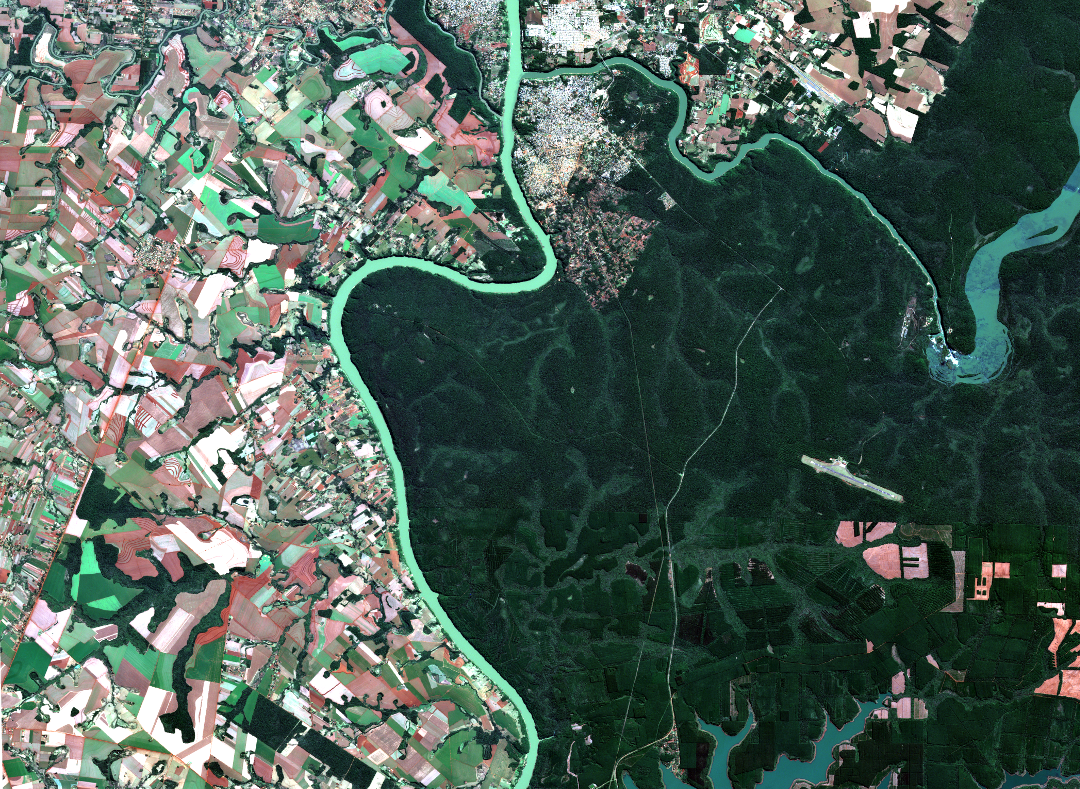
\includegraphics[scale=0.5]{fig:RVA.png}
    \caption{Imagen en combinación de colores de color real.}
    \label{fig:RVA}
\end{figure}


\section{Consulta de píxel}

Haciendo click en la pestaña \emph{Pixel info}, junto al \emph{Product explorer}, es posible obtener la información sobre un píxel para todas las bandas que se encuentren abiertas. Para utilizarla haga click en ella y posicionese sobre un píxel en la imagen (Figura \ref{fig:pixel}).

\begin{figure}[h!]
    \centering
    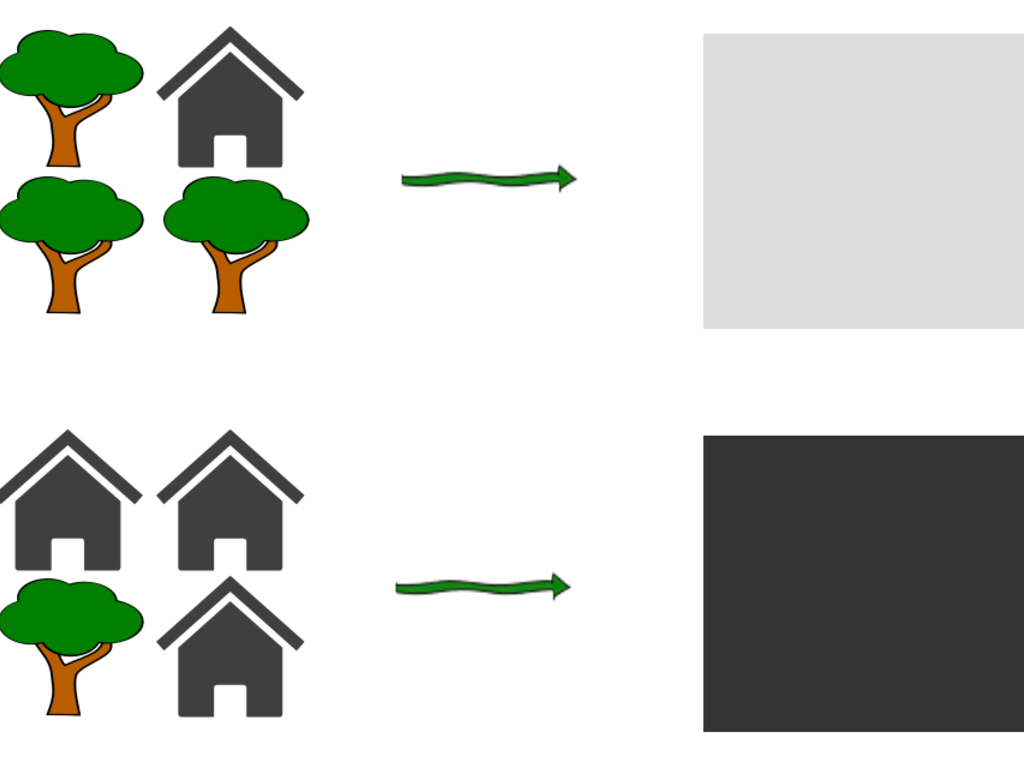
\includegraphics[width=0.3\textwidth]{fig:pixel.png}
    \caption{}
    \label{fig:pixel}
\end{figure}

Obsevará información que incluye el píxel en el que se encuentra, la latitud y longitud del píxel, las coordenadas dentro del mapa y el valor de la bandas que se encuentren abiertas.

\section{Exportar pantalla}

Es posible exportar la visualización de la pantalla del SNAP para ser abierta en distintos software.

En el caso de querer abrirla imagen en Google Earth ingrese al menú \emph{File, Export, Other, View as KMZ}. Seleccione donde quiere guardar el archivo y obtendrá un archivo \path{.kmz}.

Para abrir la imagen en otro software de GIS o exportar una imagen jpg ingrese al menú \emph{File, Export, Other, View}. En este caso deberá seleccionar el tipo de archivo en \emph{File of type}. En caso de querer mantener la georreferencia debe seleccionar el tipo \emph{GeoTIFF - TIFF with geo-location} (Figura \ref{fig:export}). Conviene elegir en este caso elegir la opción \emph{Full resolution} para mantener la resolución original de la imagen.
.

\begin{figure}[h!]
    \centering
    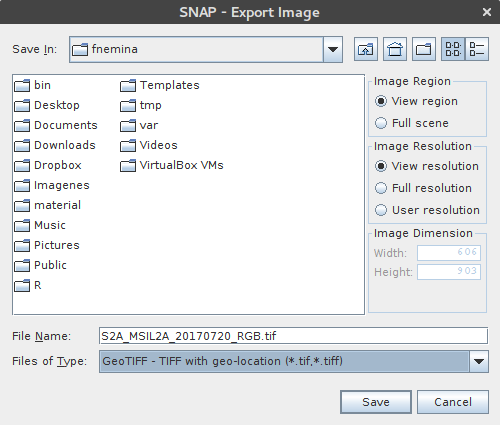
\includegraphics{fig:export.png}
    \caption{Menu para exportar vista como archivo. Incluye las opciones para elegir el recorte, la resolución y el tipo de dato de saalida.}
    \label{fig:export}
\end{figure}

\section{Actividad}

Abrá la imagen que se encuentra en la carpeta la  carpeta \path{material/raster_data/COSMO}. Abra la banda \path{Sigma0_VH}.

\begin{que}
    ¿A que coberturas dentro de la imagen pertenecen las regiones de la imagen con mayor nivel de brillo?
\end{que}

\begin{que}
    ¿Como es el valor de brillo para las zonas de cuerpos de agua?
\end{que}

\begin{que}
    ¿Cuales son las coordenadas aproximadas del aeropuerto que se encuentra en el centro de la imagen?
\end{que}
